\section{Introduction}
\label{sec1}

When generating executable code from models by applying (sequences of) model transformations, the properties modeled initially in the source model have to be propagated to the target implementation.
In general, the target implementation is more complex, due to added implementation details, which makes its analysis more difficult, more time consuming, and in some cases even impossible, as described in Chapter~\ref{chap:exploring-boundaries}.
The source model, however, is relatively small, so its properties can be inspected and validated.
To check preservation of properties, one can analyze all or some of the intermediate models, but this means that a large portion of the analysis has to be duplicated.
In addition, this procedure has to be repeated for every new model, even if only small changes to the model have been made.

The efficient and general solution to this problem is to prove property preservation per transformation and to localize the proof only on the changes induced by the transformation.
In this chapter, we address research question \RQ{4} by presenting an approach that provides such a solution.

\RQFour

Our approach is demonstrated on \SLCO, the small but non-trivial domain-specific modeling language (DSML) introduced in Chapter~\ref{chap:SLCO}.
\SLCO is a DSML for the specification of systems consisting of objects that operate in parallel and communicate with each other.
In \SLCO, such systems can be specified on various levels of abstraction.
From a given \SLCO model on a high level of abstraction, different compositions of model transformations are used to generate NQC~\cite{Baum2003} models for execution on Lego Mindstorms controllers, POOSL~\cite{Theelen2007} models for simulation, and Promela models for formal verification using the model checker SPIN~\cite{Holzmann2003}.
The transformations from \SLCO to these languages are described in Section~\ref{sec:slco:exogenous}.
The part of \SLCO used for the specification of high-level models and the three target languages have different properties, and therefore, several semantic gaps need to be bridged~\cite{Amstel2008}, which are described in Section~\ref{sec:slco:language-gaps}.
Each of these gaps is bridged by one or more model transformations that add implementation details to the original \SLCO model, resulting in a refined \SLCO model that is closer to one of the target languages.
To improve the reusability of these transformations and to deal with only one language for the majority of the correctness proofs, we only use endogenous transformations for the refinement of models, instead of exogenous ones~\cite{Mens:2006:TMT:1706639.1706924}.
These endogenous transformations are described in Section~\ref{sec:slco:endogenous}.
To be able to use endogenous transformations for refinement, we extended \SLCO with constructs to specify systems on a lower level of abstraction too.

\begin{figure}[hbt]
\centering
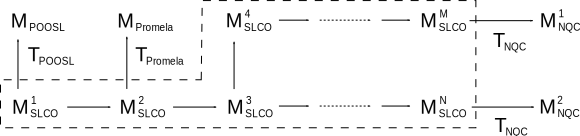
\includegraphics[width=.7\textwidth]{reusable-correct-transformations/figs/sequences}
\caption{Sequences of transformations for three target languages}
\label{fig:reusable-correct-transformations:sequences}
\end{figure}

Figure~\ref{fig:reusable-correct-transformations:sequences} schematically depicts a number of composed model transformations that transform an \SLCO model to various target languages.
The arrows inside the dashed shape depict endogenous transformations that transform \SLCO models into more refined \SLCO models.
Each of the endogenous transformations leads to a model with observationally equivalent behavior.
The arrows across the border of the dashed shape depict exogenous transformations.
Because the semantic gaps between \SLCO and the target languages are bridged completely by the endogenous transformations, these exogenous transformations are straightforward translations of \SLCO constructs into equivalent constructs in the target languages.
By developing sequences of endogenous transformations that are as fine-grained as possible, we improve the reusability of the individual transformations within sequences and reduce the number of complicated proofs.

In this chapter, we discuss how the transformations of \SLCO models to the three target languages are decomposed into sequences of transformations,
and the way these transformations are composed and reused within the sequences.
Furthermore, we describe a formal framework for \SLCO used to reason about the correctness of model transformations.
First, the formal structural operational semantics (SOS)~\cite{SOS2004Plotkin} of \SLCO is defined, which generates a labeled transition system~(LTS) representation of the dynamics of an \SLCO model.
The semantics described in this chapter are based on our experience with the executable prototype described in Chapter~\ref{chap:prototype-semantics} and describe the behavior of an \SLCO model in terms of the behavior of the individual transitions of state machines in the model.
Second, for each transformation, a (behavioral) equivalence relation is established between the behavior of an \SLCO model before and after transformation.
Finally, a proof of the correctness of a transformation is given by showing that the transformation preserves the corresponding equivalence relation.

The benefits of this approach are manifold.
The correctness of the aforementioned model transformations is proven in general, not only for particular model instances.
The use of SOS and the behavioral equivalence relations allows us to focus only on the part of a model affected by a transformation when reasoning about the correctness of this transformation.
%Here, additional benefits of fine-grained transformations are evident, since they allow for rather straightforward proofs.
Furthermore, the constraints on input models required for some of the transformations, detected earlier during experimental work, can now be formally shown necessary for the correctness of the transformations.
This proves that a sequence of transformations is well-composed if each of the intermediate models satisfies the constraints that must hold for the transformation that is applied next.

The remainder of this chapter is structured as follows.
In Section~\ref{sec:reusable-correct-transformations:model_transformations}, the model transformations related to \SLCO and the way they are reused are described.
The correctness criterion and a proof of one of the transformations are given in Section~\ref{sec:reusable-correct-transformations:correctness_of_transformations}.
This section also describes the formal semantics of \SLCO, which is required for the proof.
Section~\ref{sec:reusable-correct-transformations:related_work} discusses the related work,
and Section~\ref{sec:reusable-correct-transformations:conclusions} concludes this chapter.
